\documentclass[12pt,a4paper]{scrartcl}
    \usepackage[utf8]{inputenc}
    \usepackage{amsmath}
    \usepackage{amsfonts}
    \usepackage{amssymb}
    \usepackage{graphicx}

    \usepackage[bottom = 1in, left = 0.5in, right = 0.5in, top = 1in]{geometry}

    \usepackage[english]{babel}
    \usepackage[autostyle]{csquotes}
    \usepackage{mathptmx}

    \usepackage[labelfont=bf]{caption}

    \usepackage[default, scale=0.95]{opensans}

    \usepackage[T1]{fontenc}

    \usepackage{fixltx2e}

    % \addto\captionsenglish{\renewcommand{\figurename}{Supplementary Fig.}}
    % \addto\captionsenglish{\renewcommand{\tablename}{Supplementary Table}}

    \title{Figures}
    \date{}

\begin{document}
\maketitle

\begin{figure}[h]
	\centering
	\includegraphics[scale = 1]{../../../graphs/fig1.pdf}
	\caption{Locations of the ice stations sampled during the Transsiz expedition. Bathymetry data from the International Bathymetric Chart of the Arctic Ocean (IBCAO, v3.0).}
\end{figure}

\clearpage
\newpage

\begin{figure}[h]
	\centering
	\includegraphics[scale = 1]{../../../graphs/fig2.pdf}
	\caption{Density plots showing the distribution of transmittance values measured by the ROV and the SUIT devices. Dashed lines represent the 10\% transmittance threshold used to filter out SUIT transmittance used in the mixing models. Numbers on top of the gray boxes identify the stations.}
\end{figure}

\clearpage
\newpage

\begin{figure}[h]
	\centering
	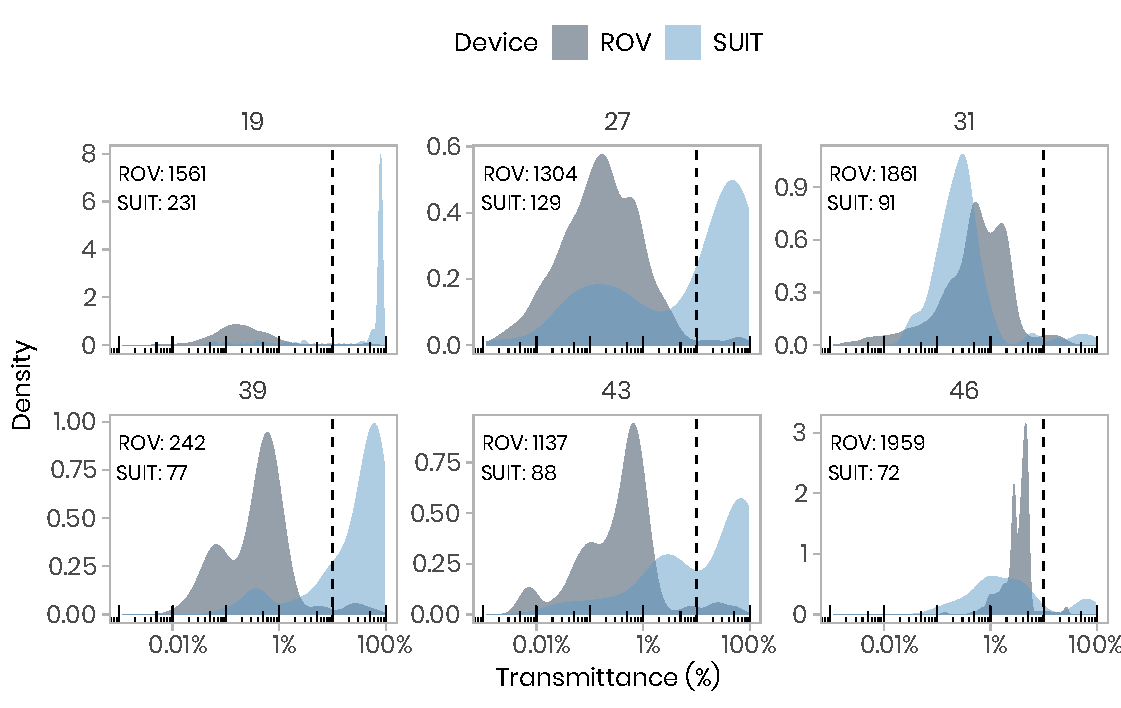
\includegraphics[scale = 1]{../../../graphs/fig3.pdf}
	\caption{Averaged vertical profiles of daily primary production. For SUIT data, mixing models were calculated using only transmittance $\le$ 0.1 whereas the under ice models were calculated using all transmittance data. Note the varying scales among stations. Numbers on top of the gray boxes identify the stations.}
\end{figure}

\clearpage
\newpage

\begin{figure}[h]
	\centering
	\includegraphics[scale = 1]{../../../graphs/fig4.pdf}
	\caption{Violin plots of primary production calculated from ROV and SUIT transmittance data. For SUIT data, mixing models were calculated using only transmittance~$\le$~10\% (see Fig. 2) whereas the under ice models were calculated using all transmittance data. Black dots inside the violin plots indicate the average primary production. Numbers on top of the gray boxes identify the stations.}
\end{figure}

\clearpage
\newpage

\begin{figure}[h]
	\centering
	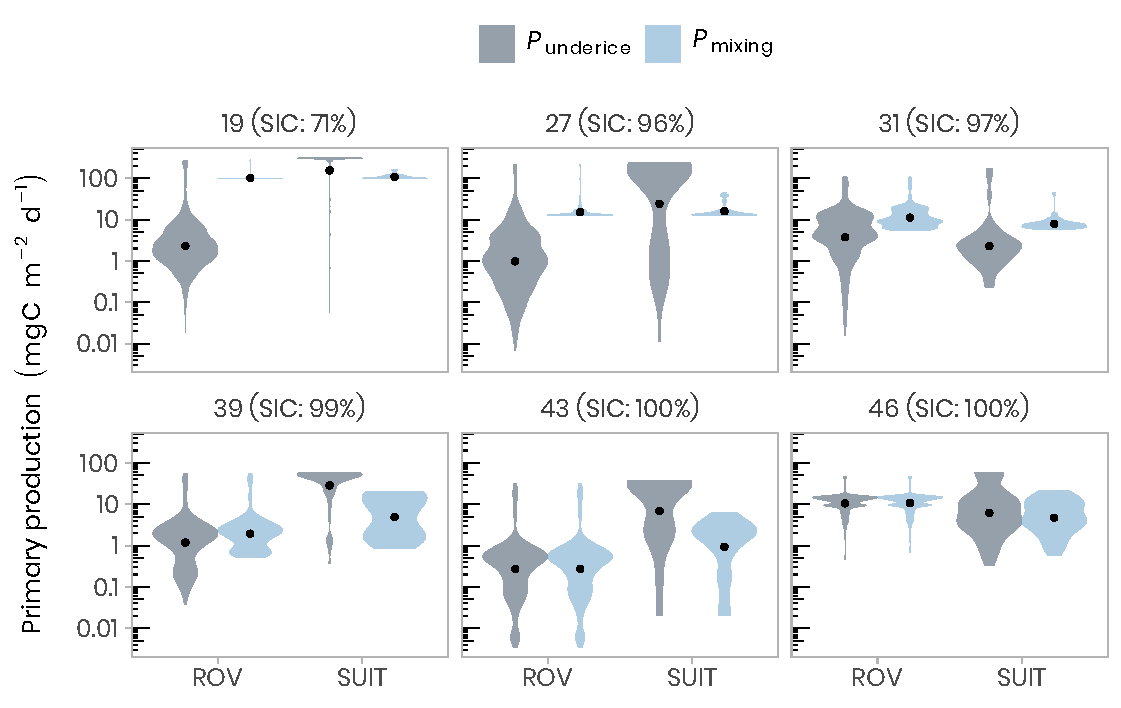
\includegraphics[scale = 1]{../../../graphs/fig5.pdf}
	\caption{Distributions of the relative errors corresponding to the absolute deviation of each individual primary estimations from the average. The red dashed lines and the numbers on the left indicate the mean errors.}
\end{figure}

\clearpage

\begin{figure}[h]
	\centering
	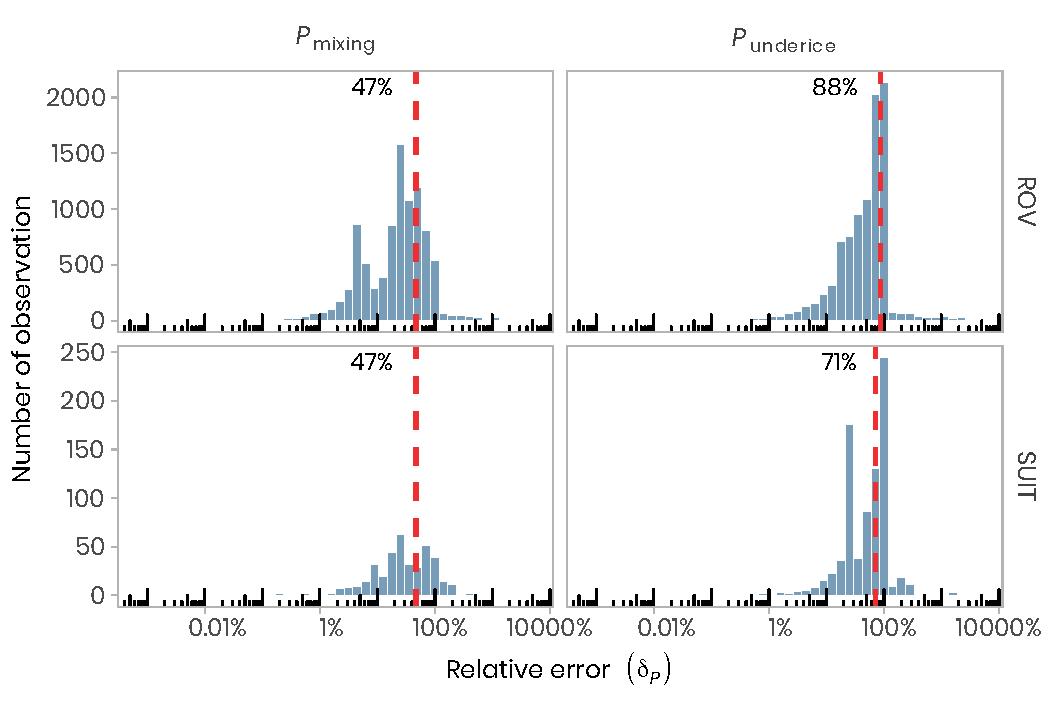
\includegraphics[scale = 1]{../../../graphs/fig6.pdf}
	\caption{Relative errors based on the number of measurements made of primary production (black dots). The shaded gray areas represent the standard deviation around the mean. The means and standard deviations were calculated from 100 randomly choosen replicates.}
\end{figure}


\end{document}
